\documentclass[11pt,a4paper,titlepage]{article}
\usepackage[utf8]{inputenc}
\usepackage[english,polish]{babel}
\usepackage[T1]{fontenc}
\usepackage{polski}
\usepackage[math,light]{anttor}
\usepackage{amsmath}
\usepackage{amsfonts}
%\usepackage{amssymb}
\usepackage{graphicx}
\usepackage{sidecap}
%\usepackage{wrapfig}
\usepackage{epstopdf}
\usepackage{booktabs}
\usepackage{forloop}
\usepackage[left=3cm,right=3cm,top=3cm,bottom=3cm]{geometry}
\usepackage[framed,numbered,autolinebreaks]{mcode}
\usepackage[colorlinks=false,urlcolor=blue,citecolor=green]{hyperref}
\usepackage{fancyhdr}
\usepackage{lastpage}
\usepackage{array}
\usepackage{hhline}
\usepackage{svg}
\usepackage{multirow}
\usepackage{enumerate}%[I], numerki, [(a)]
%ustawienie poziomów wypunktowania do wyboru: $\bullet$, $\cdot$, $\diamond$, $-$, $\ast$ and $\circ$ 
\renewcommand{\labelitemi}{$\diamond$}
\renewcommand{\labelitemii}{$\bullet$}
\renewcommand{\labelitemiii}{$-$}
\renewcommand{\labelitemiv}{$\ast$}


\AtBeginDocument{

	\renewcommand{\tablename}{Tabela}

	\renewcommand{\figurename}{Rys.}
}

%tabelki
\usepackage{tabularx}
\newcolumntype{A}{>{\centering\arraybackslash}X}
\newcolumntype{B}{>{\centering\arraybackslash} m{0.4\textwidth} }


% --- < bibliografia > ---
\usepackage[
style=numeric,
sorting=none,
% Zastosuj styl wpisu bibliograficznego właściwy językowi publikacji.
language=auto,
autolang=other,
% Zapisuj datę dostępu do strony WWW w formacie RRRR-MM-DD.
urldate=iso8601,
% Nie dodawaj numerów stron, na których występuje cytowanie.
backref=false,
% Podawaj ISBN.
isbn=true,
% Nie podawaj URL-i, o ile nie jest to konieczne.
url=false,
% Ustawienia związane z polskimi normami dla bibliografii.
maxbibnames=3,
% Jeżeli używamy BibTeXa:
backend=bibtex
]{biblatex}
% --- < bibliografia > --- Koniec

\usepackage{csquotes}
\DeclareQuoteAlias{croatian}{polish} % Ponieważ `csquotes` nie posiada polskiego stylu, można skorzystać z mocno zbliżonego stylu chorwackiego.

\addbibresource{bibliografia.bib}

\pagestyle{fancy}
\fancyhf{}
\fancyhead[R]{Segway}
\fancyfoot[R]{Optymalizacja w Systemach Sterowania}
\fancyhead[L]{M. Kowalczyk i M. Podsiadło}     
\fancyfoot[L]{Strona \thepage \hspace{1pt} z\hspace{1pt} \pageref*{LastPage}}    
\renewcommand{\headrulewidth}{1pt}
\renewcommand{\footrulewidth}{1pt}



\begin{document}
\begin{titlepage}

\newcommand{\HRule}{\rule{\linewidth}{0.5mm}} % Defines a new command for the horizontal lines, change thickness here

\center % Center everything on the page
 
%----------------------------------------------------------------------------------------
%	HEADING SECTIONS
%----------------------------------------------------------------------------------------

\textsc{\LARGE Akademia Górniczo - Hutnicza im. Stanisława Staszica}\\[0.5cm]

\includegraphics[scale=0.6]{agh}\\[1cm] % Name of your university/college
\textsc{\Large Wydział Elektrotechniki, Automatyki, Informatyki i Inżynierii Biomedycznej}\\[0.5cm] % Major heading such as course name
\textsc{\large Kierunek: Automatyka i robotyka}\\[0.5cm] % Minor heading such as course title

%----------------------------------------------------------------------------------------
%	TITLE SECTION
%----------------------------------------------------------------------------------------

\HRule \\[0.4cm]
{ \huge \bfseries Optymalizacja w Systemach Sterowania\\[1cm]Segway}\\[0.4cm] % Title of your document
\HRule \\[2cm]%[3.5cm]
 


%----------------------------------------------------------------------------------------
%	DATE SECTION
%----------------------------------------------------------------------------------------

{\large czerwiec 2017}\\[1.5cm] % Date, change the \today to a set date if you want to be precise

%----------------------------------------------------------------------------------------
%	LOGO SECTION
%----------------------------------------------------------------------------------------

%
\includegraphics[height=70mm]{agh.jpg}%\\[1cm] % Include a department/university logo - this will require the graphicx package
%----------------------------------------------------------------------------------------
%	AUTHOR SECTION
%----------------------------------------------------------------------------------------

\begin{flushleft}
\Large
\emph{Wykonali:}\\
Marcin Kowalczyk\\
Maciej Podsiadło\\[1cm]

% If you don't want a supervisor, uncomment the two lines below and remove the section above
 \emph{Prowadzący:}\\
dr hab. inż. prof. AGH Adam Korytowski\\[3cm] % Your name
 
\end{flushleft}
%----------------------------------------------------------------------------------------
\end{titlepage}
\clearpage
\setcounter{page}{2}

\clearpage
\tableofcontents
\clearpage

\section{Wstęp}
\label{sec:wstep}

Celem pracy jest numeryczne wyznaczenie optymalnego sterowania dla zadania sterowania elektryczną deskorolką lub pojazdem typu \textit{Segway}. Składają się one z platformy i dwóch kół umieszczonych z boków. Pasażer stoi na platformie. Temat uznano za szczególnie ciekawy ze względu na stale rosnącą popularność Segwayów. Pierwszy tego typu pojazd został komercyjnie sprzedany w 2002 roku za kwotę 100 tys. amerykańskich dolarów! Dzisiaj użytkowników Segwayów możemy zobaczyć praktycznie wszędzie, zaczynając od pracowników supermarketów, a kończąc na turystach sprawnie poruszających się po najbardziej zatłoczonych ulicach miasta. Jego ogromną zaletą jest możliwość poruszania na zewnątrz, jak również wewnątrz większych budynków i hal. Obecnie trwają prace nad przystosowaniem Segwaya do transportu ludzi niepełnosprawnych. Brano pod uwagę również możliwość zdalnego transportu obiektu za pomocą tego urządzenia. W tym wypadku zamiast pasażera na platformie znajdowałby się ładunek. Efektem sterowania ma być przesunięcie urządzenia do zadanego punktu w przestrzeni jednowymiarowej (początkowo zakłada się ruch w przód i w tył) oraz dwuwymiarowej (koła mają różną prędkość obrotową). Jego położenie kątowe stabilizowane jest w niestabilnym punkcie równowagi (pionowo w górę). Trudności w sterowaniu są spowodowane nieliniowością dynamiki obiektu. Kryterium do oceny stanowić może zużycie energii, czas potrzebny do osiągnięcia pozycji lub dokładność osiągniętej pozycji po zadanym czasie. %Zaproponowane sterowanie postanowiono porównać z klasycznym podejściem, wykorzystującym regulator typu PID.

\begin{figure}[h]
	\centering
	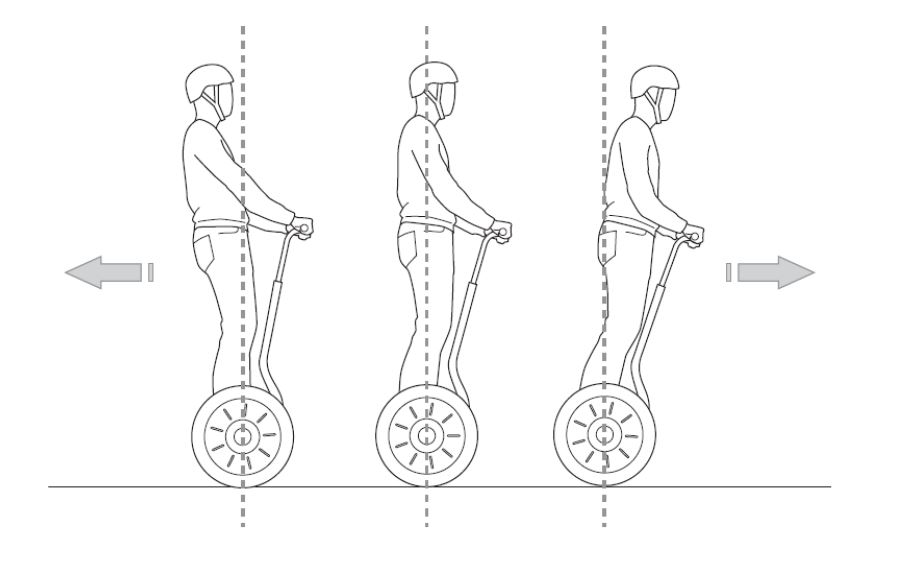
\includegraphics[width=4in]{Figures/wstep_segway.jpg}
	\captionsource{Działanie pojazdu \textit{Segway}.}{\cite{Babazadeh}}
	\label{fig:wstep_segway}
\end{figure}

Zadanie to wymaga wyznaczenia modelu matematycznego badanego obiektu oraz przetestowania jego działania. Następnie, na podstawie modelu, należy wyznaczyć optymalne sterowanie.

\appendix
\nocite{*}
\printbibliography
\addcontentsline{toc}{section}{Bibliografia}
\end{document}